\section{Бинаризация признаков}

Бинаризация признаков – это процесс преобразования исходных признаков в бинарные переменные, которые принимают значения \(0\) или \(1\). 
%Этот метод широко используется в задачах %машинного обучения, особенно в логических %методах классификации, где входные данные %должны быть представлены в виде набора %булевых предикатов.

\subsection{Бинаризация количественных признаков}

Для признака \( f: X \to D_f \), где \( D_f \) – множество возможных значений признака, бинаризация заключается в создании предикатов, проверяющих выполнение определённых условий. Эти предикаты позволяют разбить множество значений признака на подмножества, которые можно использовать в логических моделях.

В зависимости от типа признака, бинаризация осуществляется следующим образом:
\begin{itemize}
    \item \textbf{Номинальный признак} (\(f\) принимает конечное множество значений, без упорядоченности):
    \[
    \beta(x) = [f(x) = d], \quad d \in D_f;
    \]
    \[
    \beta(x) = [f(x) \in D'], \quad D' \subset D_f.
    \]
    \item \textbf{Порядковый или количественный признак} (\(f\) принимает значения, между которыми можно определить порядок):
    \[
    \beta(x) = [f(x) \leq d], \quad d \in D_f;
    \]
    \[
    \beta(x) = [d \leq f(x) \leq d'], \quad d, d' \in D_f, \, d < d'.
    \]
\end{itemize}

Для количественных признаков (\(f: X \to \mathbb{R}\)) важно выбирать такие пороговые значения \(d\), которые разделяют выборку на значимые группы. Например, 
%пороги \(d\) могут быть определены как средние значения между %соседними элементами вариационного ряда \(f(x_1), \dots, %f(x_\ell)\), упорядоченного по возрастанию:
\[
d_i = \frac{f^{(i)} + f^{(i+1)}}{2}, \quad f^{(i)} \neq f^{(i+1)}, \; i = 1, \dots, \ell - 1,
\]
где \(f^{(1)} \leq f^{(2)} \leq \dots \leq f^{(\ell)}\) – упорядоченные значения признака. (См. рис)

Такими способами можно получить много разных предикатов. Мы хотим выбрать из них самые ''лучшие'' (в каком-либо смысле). Для этого разобьем диапазон значений признака на зоны.

\begin{figure}
    \centering
    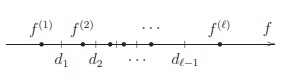
\includegraphics[scale = 1]{images/bin1.png}
    \caption{Вариационный ряд значений признака $f(x)$ и пороги $d_i$}
\end{figure}

\subsection{Разбиение диапазона значений признака на зоны}

Каждая зона определяется бинарным предикатом:
\begin{align*}
\zeta_0(x) &= [f(x) < d_1], \\
\zeta_s(x) &= [d_s \leq f(x) < d_{s+1}], \quad s = 1, \dots, r-1, \\
\zeta_r(x) &= [d_r \leq f(x)].
\end{align*}

Способы разбиения:
\begin{itemize}
    \item Жадная максимизация информативности путем слияний
    \item Разбиение на равномощные подвыборки
    \item Разбиение по равномерной сетке ''удобных'' значений (например, с минимальным числом значащих цифр)
    \item Объединение нескольких разбиений
\end{itemize}

\subsection{Жадный алгоритм слияния зон}

Алгоритм начинает с разбиения на ''мелкие'' зоны. Пороги проходят между всеми соседними парами точек, принадлежащих \emph{разным} классам, т.~к. расстановка порогов между точками одного класса приведет только к уменьшению информативности зон. Далее зоны укрупняются путём слияния \emph{троек} соседних зон. Зоны сливаются до тех пор, пока
информативность некоторой слитой зоны превышает информативность
исходных зон, либо пока не будет получено заданное количество зон $r$. Каждый раз сливается тройка, дающая наибольший выигрыш в информативности.

\begin{figure}
    \centering
    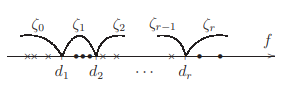
\includegraphics[scale = 1]{images/bin2.png}
    \caption{Начальное разбиение на зоны}
\end{figure}

\newpage
\textbf{Вход:}
\begin{itemize}
    \item $f(x)$ — признак;
    \item $c \in Y$ — выделенный класс;
    \item $X^\ell = \{(x_i, y_i)\}_{i=1}^\ell$ — выборка, упорядоченная по возрастанию $f(x_i)$;
    \item $r$ — желаемое количество зон;
    \item $\delta_0$ — порог слияния зон (по умолчанию $\delta_0 = 0$).
\end{itemize}

\textbf{Выход:}
\[
D = \{d_1, \dots, d_n\} \text{ — строго возрастающая последовательность порогов;}
\]

\hline

\begin{enumerate}
    \item $D := \emptyset;$
    \item \textbf{для всех} $i = 2, \dots, \ell$:
    \begin{itemize}
        \item \textbf{если} $f(x_{i-1}) \neq f(x_i)$ и $[y_{i-1} = c] \neq [y_i = c]$ \textbf{то}
        \begin{itemize}
            \item добавить новый порог $d := \frac{f(x_{i-1}) + f(x_i)}{2}$ в конец последовательности $D$;
        \end{itemize}
    \end{itemize}
    \item \textbf{повторять}
    \begin{enumerate}
        \item \textbf{для всех} $d_i \in D, i = 1, \dots, |D| - 1$:
        \begin{itemize}
            \item вычислить выигрыш от слияния тройки соседних зон $\zeta_{i-1}, \zeta_i, \zeta_{i+1}$:
            \[
            \delta_i := I_c(\zeta_{i-1} \cup \zeta_i \cup \zeta_{i+1}) - \max\{I_c(\zeta_{i-1}), I_c(\zeta_i), I_c(\zeta_{i+1})\};
            \]
        \end{itemize}
        \item найти тройку зон, для которой слияние наиболее выгодно:
        \[
        i := \arg \max \delta_i;
        \]
        \item \textbf{если} $\delta_i > \delta_0$ \textbf{то}
        \begin{itemize}
            \item слить зоны $\zeta_{i-1}, \zeta_i, \zeta_{i+1}$, удалить пороги $d_i$ и $d_{i+1}$ из последовательности $D$;
        \end{itemize}
    \end{enumerate}
    \item \textbf{пока} $|D| > r + 1$.
\end{enumerate}

\subsection{Задачи}

\textbf{Задача 1}
Предположим, вы владелец интернет-магазина, и у вас есть данные о стоимости товаров и их популярности (популярен — \( 1 \), непопулярен — \( 0 \)). 
Для анализа спроса вы хотите разбить товары на ценовые зоны, чтобы лучше понять поведение покупателей.

Данные представлены в таблице:

\[
\begin{array}{|c|c|c|}
\hline
\text{№ товара} & \text{Цена товара (\$)} & \text{Популярность } y \\
\hline
1 & 10 & 1 \\
2 & 12 & 1 \\
3 & 15 & 0 \\
4 & 17 & 1 \\
5 & 20 & 0 \\
6 & 23 & 0 \\
7 & 25 & 1 \\
\hline
\end{array}
\]

Как алгоритм слияния зон первично разобьёт выборку на ценовые зоны?

\textbf{Решение}
Рассчитаем пороги:

\[
\begin{aligned}
&d_1 = \frac{12 + 15}{2} = 13.5, \\
&d_2 = \frac{15 + 17}{2} = 16.0, \\
&d_3 = \frac{17 + 20}{2} = 18.5, \\
&d_4 = \frac{23 + 25}{2} = 24.0
\end{aligned}
\]

На основе рассчитанных порогов получаем зоны:

\[
\begin{aligned}
&\zeta_0(x) = [\text{Цена} < 13.5], \\
&\zeta_1(x) = [13.5 \leq \text{Цена} < 16.0], \\
&\zeta_2(x) = [16.0 \leq \text{Цена} < 18.5], \\
&\zeta_4(x) = [29.0 \leq \text{Цена} < 24.0], \\
&\zeta_5(x) = [\text{Цена} \geq 24.0].
\end{aligned}
\]

\textbf{Задача 2}
Будут ли разбиения диапазона меняться в зависимости от класса, относительно которого они производятся? Как изменить алгоритм для получения ''универсального'' разбиения, учитывающего сразу все классы? 

\textbf{Решение}
Да, будут, т.~к. информативность зависит от класса. Нужно заменить критерий информативности многоклассовым критерием.

\textbf{Задача 3}
Какую сложность имеет алгоритм слияния зон? Как можно его ускорить?

\textbf{Решение}
Этот алгоритм имеет трудоёмкость $O(l^2)$. Его можно заметно ускорить, если на каждой итерации сливать не одну тройку зон, а $\tau l$ троек с достаточно большим выигрышем $\delta I_i$, при условии, что они не перекрываются. В этом случае трудоёмкость составляет $O(l / \sqrt{\tau})$.

\section{Взвешенное голосование правил}

Допустим, имеется консилиум экспертов, каждый член которого может допустить ошибку. Процедура голосования — это способ повышения качества принимаемых решений, при котором ошибки отдельных экспертов компенсируют друг друга.

Ранее принцип голосования применялся для построения композиций из произвольных алгоритмов классификации. Теперь рассмотрим композиции, состоящие из логических закономерностей.

\subsection{Принцип голосования}

Пусть для каждого класса $c \in Y$ построено множество логических закономерностей (правил), специализирующихся на различении объектов данного класса:

\[
R_c = \{ \varphi_{tc} : X \to \{0, 1\} \mid t = 1, \dots, T_c \}
\]

Считается, что если $\varphi_{tc}(x) = 1$, то правило $\varphi_{tc}$ относит объект $x \in X$ к классу $c$. Если же $\varphi_{tc}(x) = 0$, то правило воздерживается от классификации объекта $x$.

Алгоритм простого голосования (simple voting) подсчитывает долю правил в наборах $R_c$, относящих объект $x$ к каждому из классов:

\[
\Gamma_c(x) = \frac{1}{T_c} \sum_{t=1}^{T_c} \varphi_{tc}(x), \quad c \in Y,
\]

и относит объект $x$ к тому классу, за который подана наибольшая доля голосов:

\[
a(x) = \arg \max_{c \in Y} \Gamma_c(x).
\]

Если максимум достигается одновременно на нескольких классах, выбирается тот, для которого цена ошибки меньше.

Нормирующий множитель $\frac{1}{T_c}$ вводится для того, чтобы наборы с большим числом правил не перетягивали объекты в свой класс.

\subsection{Алгоритм взвешенного голосования}
Алгоритм взвешенного голосования (weighted voting, WV) действует более тонко, учитывая, что правила могут иметь различную ценность. Каждому правилу $\varphi_{tc}$ приписывается вес $\alpha_{tc} \geq 0$, и при голосовании берется взвешенная сумма голосов:

\[
\Gamma_c(x) = \sum_{t=1}^{T_c} \alpha_{tc} \varphi_{tc}(x), \quad \alpha_{tc} > 0.
\]

Веса нормируются на единицу:

\[
\sum_{t=1}^{T_c} \alpha_{tc} = 1, \quad \forall c \in Y.
\]

Поэтому функцию $\Gamma_c(x)$ называют также выпуклой комбинацией правил $\varphi_1, \dots, \varphi_{T_c}$. Очевидно, простое голосование является частным случаем взвешенного, когда веса одинаковы и равны $\frac{1}{T_c}$.

На первый взгляд, вес правила должен определяться его информативностью. Однако, важно также учитывать, насколько данное правило уникально. Если имеется 10 хороших, но одинаковых (или почти одинаковых) правил, их суммарный вес должен быть сравним с весом столь же хорошего правила, не похожего на все остальные. Таким образом, веса должны учитывать не только ценность правил, но и их различность.

Простой общий подход к настройке весов заключается в том, чтобы сначала найти набор правил $\{ \varphi_{tc}(x) \}$, затем принять их за новые (бинарные) признаки и построить в этом новом признаковом пространстве линейную разделяющую поверхность (кусочно-линейную, если $|Y| > 2$). Для этого можно использовать логистическую регрессию, однослойный персептрон или метод опорных векторов. Существуют и другие подходы. Например, в разделе 1.5.4 будет рассмотрен метод бустинга, в котором правила настраиваются последовательно, и для каждого правила сразу вычисляется его вес.

\subsection{Проблема диверсификации правил}
Голосующие правила должны быть существенно различны, иначе они будут бесполезны для классификации. Продолжая аналогию с консилиумом, заметим, что нет никакого смысла держать в консилиуме эксперта A, если он регулярно подсматривает решения у эксперта B.

Приведем простое теоретико-вероятностное обоснование принципа диверсификации, или повышения различности (diversity) правил \cite{14}. Пусть $X$ — вероятностное пространство, множество ответов $Y$ конечно. Введем случайную величину $M(x)$, равную перевесу голосов в пользу правильного класса; её называют также отступом (margin) объекта $x$ от границы классов:

\[
M(x) = \Gamma_c(x) - \Gamma_{\overline{c}}(x), \quad \Gamma_{\overline{c}}(x) = \max_{y \in Y \setminus \{c\}} \Gamma_y(x), \quad c = y^*(x).
\]

Если отступ положителен ($M(x) > 0$), то алгоритм голосования правильно классифицирует объект $x$. Предположим, что в среднем наш алгоритм классифицирует хотя бы немного лучше, чем наугад: $E[M] > 0$. Тогда можно оценить вероятность ошибки по неравенству Чебышева:

\[
P\{M < 0\} \leq P\{|E[M] - M| > E[M]\} \leq \frac{D_M}{(E[M])^2}.
\]

Отсюда вывод: для уменьшения вероятности ошибки необходимо максимизировать ожидание перевеса голосов $E[M]$ и минимизировать его дисперсию $D_M$. Для выполнения этих условий каждый объект должен выделяться примерно одинаковым числом правил. Обычно ни одно из правил не выделяет класс целиком, поэтому правила должны быть существенно различны, то есть выделять существенно различные подмножества объектов.

Неплохая эвристика, усиливающая различия между правилами и позволяющая равномернее выделять объекты обучения, используется в алгоритме CORAL \cite{12}. Сначала для фиксированного класса $c \in Y$ строится покрывающий набор правил точно так, как это делалось для решающих списков. Затем строится второй покрывающий набор, но при этом запрещается использовать признаки, часто входившие в закономерности первого набора. Поэтому второй набор неминуемо окажется отличным от первого. Затем запрещаются признаки, часто входившие в оба набора, и строится третий набор. И так далее, для каждого класса $c \in Y$.

\subsection{Отказы от классификации}
Возможны ситуации, когда ни одно из правил не выделяет классифицируемый объект $x$. Тогда алгоритм должен либо отказываться от классификации, либо относить объект к классу, имеющему наименьшую цену ошибки. Отказ алгоритма означает, что данный объект является нетипичным, не подпадающим ни под одну из ранее обнаруженных закономерностей. Вообще, обнаружение нетипичности (novelty detection) принято считать отдельным видом задач обучения по прецедентам, наряду с классификацией и кластеризацией. Способность алгоритмов отказываться от классификации нетипичных объектов во многих приложениях является скорее преимуществом, чем недостатком. В то же время, число отказов не должно быть слишком большим.

Итак, при построении алгоритмов взвешенного голосования правил возникает четыре основных вопроса:
\begin{itemize}
    \item Как построить много правил по одной и той же выборке?
    \item Как избежать повторов и построения почти одинаковых правил?
    \item Как избежать появления непокрытых объектов и обеспечить равномерное покрытие всей выборки правилами?
    \item Как определять веса правил при взвешенном голосовании?
\end{itemize}

Рассмотрим, как эти проблемы решаются в известных алгоритмах в следующих параграфах.

\subsection{Задачи}

\textbf{Задача 1: Алгоритм простого голосования}

Допустим, для класса $c \in Y$ существуют 10 правил, которые используют данные для классификации. Каждое правило возвращает 1 или 0 для объекта $x$. Если для объекта $x$ правила 3 и 7 верно классифицируют объект как класс $c$, а остальные возвращают 0, как будет рассчитана доля голосов для класса $c$?

\textbf{Решение:}  
Для класса $c$ доля голосов рассчитывается как сумма всех правил, которые классифицируют объект как класс $c$, делённая на общее количество правил. Если 10 правил, то:
\[
\Gamma_c(x) = \frac{1}{10} \left( 1 + 0 + 0 + 0 + 0 + 0 + 1 + 0 + 0 + 0 \right) = \frac{2}{10} = 0.2
\]
Таким образом, для объекта $x$ доля голосов для класса $c$ составит 0.2.

\textbf{Задача 2: Проблема с весами в алгоритме взвешенного голосования}

В алгоритме взвешенного голосования веса для каждого правила нормируются на единицу. Если для класса $c$ у нас есть 3 правила с весами $\alpha_1 = 0.5$, $\alpha_2 = 0.3$, и $\alpha_3 = 0.2$, как будет выглядеть итоговая сумма голосов $\Gamma_c(x)$, если объект $x$ классифицируется всеми тремя правилами как класс $c$?

\textbf{Решение:}  
Итоговая сумма голосов для класса $c$ рассчитывается по формуле:
\[
\Gamma_c(x) = \sum_{t=1}^{T_c} \alpha_{tc} \varphi_{tc}(x)
\]
где $\varphi_{tc}(x) = 1$, если правило классифицирует объект как класс $c$, и 0 в противном случае. Если все 3 правила классифицируют объект как $c$, то:
\[
\Gamma_c(x) = 0.5 + 0.3 + 0.2 = 1.0
\]

\textbf{Задача 3: Проблема диверсификации правил}

Какова вероятность ошибки при использовании алгоритма голосования, если все правила сильно похожи друг на друга (например, классифицируют одинаковые подмножества объектов)?

\textbf{Решение:}  
Если правила сильно похожи, то вероятность ошибки возрастает. В таких случаях, возможно, правило не будет существенно различать объекты, и алгоритм может ошибаться при классификации новых объектов. Чтобы уменьшить вероятность ошибки, правила должны быть разнообразными, то есть они должны выделять разные подмножества объектов. Для максимизации различий между правилами можно использовать метод, как в алгоритме CORAL, который строит покрывающие наборы правил, постепенно исключая часто встречающиеся признаки.

\textbf{Задача 4: Принцип диверсификации правил}

Пусть для объекта $x$ имеется 10 правил, из которых 8 классифицируют объект как класс $c$, а остальные 2 — как класс $d$. Какой отступ $M(x)$ будет при расчете вероятности правильной классификации?

\textbf{Решение:}  
Отступ для объекта $x$ определяется как разница между голосами для правильного класса и максимальным голосом для всех остальных классов:
\[
M(x) = \Gamma_c(x) - \Gamma_{\overline{c}}(x)
\]
Если из 10 правил 8 голосуют за класс $c$ (доля голосов $0.8$) и 2 — за класс $d$ (доля голосов $0.2$), то:
\[
M(x) = 0.8 - 0.2 = 0.6
\]
Если отступ положителен ($M(x) > 0$), то классификация будет правильной.

\textbf{Задача 5: Отказы от классификации}

Если для объекта $x$ не существует правила, которое его классифицирует, что должен делать алгоритм голосования? Как можно обработать такой случай?

\textbf{Решение:}  
В таком случае алгоритм может либо отказаться от классификации, либо отнести объект к классу с наименьшей ценой ошибки. Такой отказ от классификации часто называют обнаружением нетипичности (novelty detection), что является отдельной задачей в машинном обучении. Важно, чтобы количество отказов не было слишком большим, так как это может снизить эффективность алгоритма.

\section{Алгоритм ТЭМП}

Полный перебор всех конъюнкций ранга не более $K$ требует экспоненциального по $K$ числа операций. В реальных задачах объём вычислений становится огромным уже при $K > 3$, и от идеи полного перебора приходится отказаться.

Существует две стандартные стратегии перебора конъюнкций: поиск в глубину (depth-first search) и поиск в ширину (breadth-first search). Первая применяется в алгоритме КОРА, вторая — в алгоритме ТЭМП, предложенным Г. С. Лбовым в 1976 году. Поиск в ширину работает немного быстрее, и в него легче встраивать различные эвристики, сокращающие перебор.

В исходном варианте алгоритм ТЭМП выполнял полный перебор всех конъюнкций ранга не более $K$. Ниже описан слегка модифицированный вариант, позволяющий ограничить перебор и увеличить максимальный ранг конъюнкций $K$.

Алгоритм 1.9 начинает процесс поиска закономерностей с построения конъюнкций ранга 1. Для этого отбираются не более $T_1$ самых информативных предикатов из базового множества $\mathcal{B}$. Затем к каждому из отобранных предикатов добавляется по одному терму из $\mathcal{B}$ всеми возможными способами. Получается не более $T_1|\mathcal{B}|$ конъюнкций ранга 2, из которых снова отбираются $T_1$ самых информативных. И так далее. На каждом шаге процесса делается попытка добавить один терм к каждой из имеющихся конъюнкций. Наращивание конъюнкций прекращается либо при достижении максимального ранга $K$, либо когда ни одну из конъюнкций не удаётся улучшить путём добавления терма.

Лучшие конъюнкции, собранные со всех шагов, заносятся в списки $R_c$. Таким образом, списки $R_c$ могут содержать конъюнкции различного ранга.

Параметр $T_1$ позволяет найти компромисс между качеством и скоростью работы алгоритма. При $T_1 = 1$ алгоритм ТЭМП работает исключительно быстро и строит единственную конъюнкцию, добавляя термы по очереди. Фактически, он совпадает с жадным Алгоритмом 1.2. При увеличении $T_1$ пространство поиска расширяется, алгоритм начинает работать медленнее, но находит больше информативных конъюнкций. На практике выбирают максимальное значение параметра $T_1$, при котором поиск занимает приемлемое время. Однако стратегия поиска всё равно остаётся жадной — термы оптимизируются по-отдельности, и при подборе каждого терма учитываются только предыдущие, но не последующие термы.

Для улучшения конъюнкций к ним применяют эвристические методы «финальной шлифовки» — стабилизацию и редукцию.

В результате стабилизации конъюнкции становятся локально неулучшаемыми. Алгоритм в целом становится более устойчивым — при незначительных изменениях в составе обучающей выборки он чаще находит одни и те же закономерности, а значит, улучшается его способность обобщать эмпирические факты.

В результате стабилизации некоторые конъюнкции могут совпасть, и в списке появятся дубликаты. Их удаление предусмотрено на шаге 13. Если список $R_c$ поддерживается отсортированным по информативности, то удаление дубликатов является недорогой операцией, так как достаточно проверять на совпадение только соседние конъюнкции с одинаковой информативностью.

Если задать $T_1 = \infty$, то алгоритм выполнит полный перебор, как в исходном варианте ТЭМП. «Финальная шлифовка» в этом случае не нужна.

\subsection{Алгоритм 1.9. Построение списка информативных конъюнкций методом поиска в ширину (алгоритм ТЭМП)}


\subsection{Алгоритм 1.9: Построение списка информативных конъюнкций методом поиска в ширину}

\textbf{Вход:}
\begin{itemize}
    \item $X_\ell$ --- обучающая выборка;
    \item $\mathcal{B}$ --- семейство элементарных предикатов;
    \item $c \in Y$ --- класс, для которого строится список конъюнкций;
    \item $K$ --- максимальный ранг конъюнкций;
    \item $T_1$ --- число лучших конъюнкций, отбираемых на каждом шаге;
    \item $T_0$ --- число лучших конъюнкций, отбираемых на последнем шаге, $T_0 \leq T_1$;
    \item $I_{\min}$ --- порог информативности;
    \item $E_{\max}$ --- порог допустимой доли ошибок;
    \item $X_k$ --- контрольная выборка для проведения редукции.
\end{itemize}

\textbf{Выход:} Список конъюнкций $R_c = \{\varphi_t^c(x) : t = 1, \dots, T_c\}$.

\begin{enumerate}
    \item $R_c \gets \emptyset$;
    \item Для всех $\beta \in \mathcal{B}$: \texttt{Добавить\_в\_список($R_c$, $\beta$, $T_1$)};
    \item Для всех $k = 2, \dots, K$:
    \begin{enumerate}
        \item Для всех конъюнкций $\varphi \in R_c$ ранга $(k-1)$:
        \begin{enumerate}
            \item Для всех предикатов $\beta \in \mathcal{B}$, которых ещё нет в конъюнкции $\varphi$:
            \begin{enumerate}
                \item Добавить терм $\beta$ к конъюнкции $\varphi$: $\varphi' = \varphi \land \beta$;
                \item Если $I_c(\varphi') > I_{\min}$, $E_c(\varphi') \leq E_{\max}$ и конъюнкции $\varphi'$ нет в $R_c$, то \texttt{Добавить\_в\_список($R_c$, $\varphi'$, $T_1$)}.
            \end{enumerate}
        \end{enumerate}
    \end{enumerate}
    \item Для всех конъюнкций $\varphi \in R_c$:
    \begin{enumerate}
        \item Стабилизация($\varphi$);
        \item Редукция($\varphi$, $X^k$);
    \end{enumerate}
    \item Удалить из списка $R_c$ дублирующие конъюнкции;
    \item Оставить в списке $R_c$ не более $T_0$ лучших конъюнкций.
\end{enumerate}


\subsection{Достоинства алгоритма ТЭМП}

\begin{itemize}
    \item ТЭМП существенно более эффективен, чем КОРА, особенно при поиске конъюнкций ранга больше 3. Он решает поставленную задачу за $O(KT_1|B|\\ell)$ операций, тогда как КОРА имеет трудоёмкость $O(|B|K\\ell)$.
    \item Параметр $T_1$ позволяет управлять жадностью алгоритма и находить компромисс между качеством конъюнкций и скоростью работы алгоритма.
    \item Благодаря простоте и эффективности алгоритм ТЭМП можно использовать в составе других алгоритмов как генератор конъюнкций, достаточно близких к оптимальным.
\end{itemize}

\subsection{Недостатки алгоритма ТЭМП}

\begin{itemize}
    \item Нет гарантии, что будут найдены самые лучшие конъюнкции, особенно при малых значениях параметра $T_1$.
    \item Алгоритм не стремится увеличивать различность конъюнкций, добиваясь равномерного покрытия объектов выборки. Стабилизация и редукция лишь отчасти компенсируют этот недостаток.
    \item Нет настройки коэффициентов $\\alpha_{tc}$; предполагается простое голосование.
\end{itemize}

\subsection{Задачи}

    \textbf{Задача 1.}

    \newline
    Рассмотрите граф $G = (V, E)$, где $V = \{A, B, C, D, E\}$ и $E = \{(A, B), (A, C), (B, D), (C, D), (D, E)\}$. Как алгоритм ТЭМП выполняет поиск в ширину для этого графа? Предложите, как можно выполнить поиск в глубину.

\textit{Решение:}
\begin{enumerate}
    \item Алгоритм ТЭМП начинает с вершины $A$, добавляя её соседей $B$ и $C$ в очередь. Затем из очереди выбирается вершина $B$, её сосед $D$ добавляется в очередь, и так далее.
    \item Для поиска в глубину из вершины $A$ алгоритм выбирает один путь (например, $A \to B \to D \to E$), пока не дойдёт до конца, затем возвращается и ищет другие пути.
\end{enumerate}

\textbf{Задача 2.}
\newline
Пусть у нас есть множество предикатов $B = \beta_1, \beta_2, \beta_3$ и максимальный ранг $K = 2$. Какое количество конъюнкций будет проверено алгоритмом ТЭМП, если для каждого шага выбирается $T_1 = 2$? Если мы увеличим $T_1$ до 3, как это повлияет на количество проверяемых конъюнкций?

\textit{Решение:}
\begin{itemize}
    \item При $T_1 = 2$ для ранга 1 будет 2 конъюнкции, для ранга 2 --- $2 \times 3 = 6$ конъюнкций. Всего будет проверено $2 + 6 = 8$ конъюнкций.
    \item Если $T_1 = 3$, то для ранга 1 будет 3 конъюнкции, для ранга 2 --- $3 \times 3 = 9$ конъюнкций. Всего будет проверено $3 + 9 = 12$ конъюнкций.
\end{itemize}

\textbf{Задача 3.}
\newline
Представьте, что вы используете алгоритм ТЭМП для обучения модели с большим количеством предикатов. Какой будет влияние на время вычислений, если вы увеличите $T_1$ с 1 до 5? Объясните это с точки зрения расширения пространства поиска.

\textit{Решение:}
\begin{itemize}
    \item При $T_1 = 1$ алгоритм будет проверять только по одному терму для каждой конъюнкции на каждом шаге, что будет довольно быстрым, но может не давать лучшие результаты.
    \item При увеличении $T_1$ до 5 пространство поиска расширяется, так как на каждом шаге будет добавляться больше термов к конъюнкциям, что увеличивает количество проверяемых комбинаций и тем самым замедляет процесс.
    \item В результате увеличение $T_1$ может существенно замедлить алгоритм, но при этом улучшится качество найденных решений.
\end{itemize}


\subsection*{Алгоритм бустинга}

Алгоритмы КОРА и ТЭМП имеют общий недостаток~--- они не стремятся увеличивать различность комбинаций. Эта проблема решается в алгоритме бустинга.

\textit{Бустинг} (boosting) предложили американские учёные Фройнд и Шапир как универсальный метод построения выпускной комбинации классификаторов. 

В бустинге закономерности строятся последовательно, и после построения очередной закономерности веса выделенных ею объектов изменяются~--- уменьшаются у позитивных и увеличиваются у негативных объектов. Обновлённый вектор весов $w$ у объектов $x$ определяется следующей закономерностью по критерию максимума \textit{взвешенной информации}. В результате каждая следующая закономерность стремится выделять ``наименее покрытые'' объекты, оказывающиеся ``наиболее трудными'' для предыдущих закономерностей. Это способ повышения разнообразия закономерностей, более равномерного покрытия объектов и повышения обобщающей способности выпускной комбинации закономерностей.

Описанная стратегия напоминает алгоритм построения решающего списка. Разница в том, что там было достаточно покрыть объект один раз, после чего он исключался из рассмотрения. Здесь же каждое покрытие только изменяет вес объекта.

Для реализации этой идеи остаётся понять, как именно должны изменяться веса объектов и веса закономерностей на каждом этапе алгоритма.

Рассмотрим задачу классификации с двумя классами, $Y = \{-1, +1\}$ и алгоритм взвешенного голосования, состоящий из $T = T_{-1} + T_{+1}$ закономерностей:
\begin{equation}
    a_T(x) = \text{sign}\left( \sum_{t=1}^{T_{+1}} \alpha^t_{+1} \varphi^t_{+1}(x) - \sum_{t=1}^{T_{-1}} \alpha^t_{-1} \varphi^t_{-1}(x) \right), \quad \alpha^t_c > 0, \, c \in Y.
\end{equation}

\subsection*{Экспоненциальная аппроксимация пороговой функции потерь}

Пусть уже построено $T$ закономерностей, вместе составляющих алгоритм классификации $a_T(x)$. При добавлении ещё одной закономерности $\varphi_c(x)$ в список $\mathcal{R}_c$ взвешенная сумма голосов за класс $c \in \{-1, +1\}$ примет вид
\begin{equation}
    \Gamma'_c(x) = \Gamma_c(x) + \alpha \varphi_c(x).
\end{equation}

Задача состоит в том, чтобы найти закономерность $\varphi_c$ и её вес $\alpha$, при которых алгоритм $a_{T+1}(x)$ допускает минимальное число ошибок на обучающей выборке $X^\ell$.

Число ошибок алгоритма $a_T(x)$ перед добавлением закономерности $\varphi_c$:
\begin{equation}
    Q_T = \sum_{i=1}^\ell \left[ \Gamma_{y_i}(x_i) - \Gamma_{-y_i}(x_i) < 0 \right].
\end{equation}

Число ошибок алгоритма $a_{T+1}(x)$ после добавления закономерности $\varphi_c$:
\begin{equation}
    Q_{T+1}(\varphi_c, \alpha) = \sum_{i=1}^\ell \left[ y_i = c \right] 
    \left[ \Gamma_{y_i}(x_i) - \Gamma_{-y_i}(x_i) + \alpha \varphi_c(x_i) < 0 \right] + 
    \sum_{i=1}^\ell \left[ y_i \neq c \right] 
    \left[ \Gamma_{y_i}(x_i) - \Gamma_{-y_i}(x_i) + \alpha \varphi_c(x_i) < 0 \right].
\end{equation}

Выписанный функционал содержит параметр $\alpha$ внутри пороговой функции вида $\left[ z(\alpha) < 0 \right]$, следовательно, является разрывной функцией от $\alpha$. Минимизация такого функционала является нетривиальной задачей комбинаторной оптимизации. Попробуем упростить её приближением. Заменим пороговую функцию непрерывно дифференцируемой оценкой сверху. Тогда минимизацию по $\alpha$ можно будет выполнить аналитически.

Запишем верхнюю оценку $\tilde{Q}_T$ функционала $Q_T$:
\begin{equation}
    Q_T \leq \tilde{Q}_T \equiv \sum_{i=1}^\ell \exp\left(\Gamma_{-y_i}(x_i) - \Gamma_{y_i}(x_i)\right) = \sum_{i=1}^\ell w_i.
\end{equation}

Если алгоритм $a_T(x)$ правильно классифицирует объект $x_i$, то $w_i < 1$. Если ошибается, то $w_i > 1$. Чем больше перевес голосов в пользу ошибочного класса, тем больше вес $w_i$. Таким образом, большие веса получают наиболее ``трудные'' объекты.

Введём вектор весов $w = \{w_i\}_{i=1}^\ell$ с компонентами $w_i = \ell \tilde{w}_i / \tilde{Q}_T$. Тогда будет выполнено условие нормировки $\sum_{i=1}^\ell w_i = \ell$. Следующая теорема показывает, что выбор $w_i$ в качестве весов объектов оптимален для построения $(T+1)$-й закономерности.

\textbf{Теорема 1.2.} Минимум функционала $\tilde{Q}_{T+1}(\varphi_c, \alpha)$ достигается при
\begin{equation}
    \varphi_c^* = \arg \max_{\varphi_c \in \mathcal{R}_c} J_c^w(\varphi_c, X^\ell), \quad
    J_c^w(\varphi_c, X^\ell) = \sqrt{p_c^w(\varphi_c)} - \sqrt{n_c^w(\varphi_c)},
\end{equation}
\begin{equation}
    \alpha^* = \frac{1}{2} \ln \frac{p_c^w(\varphi_c^*)}{n_c^w(\varphi_c^*)}, \quad \text{при } n_c^w(\varphi_c) \neq 0,
\end{equation}
где функции $p_c^w$ и $n_c^w$ определяются по формулам (1.3).

\textbf{Доказательство.} 

Распишем функционал $\tilde{Q}_{T+1}$, воспользовавшись тождеством $e^A = (1-\varphi) + \varphi e^A$, которое справедливо при любых $A \in \mathbb{R}$ и $\varphi \in \{0,1\}$.

\begin{equation}
    \tilde{Q}_{T+1} = \sum_{i=1}^\ell w_i e^{-\alpha \varphi_c(x_i)} \left[ y_i = c \right] 
    + \sum_{i=1}^\ell w_i e^{\alpha \varphi_c(x_i)} \left[ y_i \neq c \right] =
    \sum_{i=1}^\ell w_i (1 - \varphi_c(x_i)) + e^{-\alpha} \sum_{i=1}^\ell w_i \varphi_c(x_i) \left[ y_i = c \right] 
    + e^\alpha \sum_{i=1}^\ell w_i \varphi_c(x_i) \left[ y_i \neq c \right].
\end{equation}

Подставим в эту формулу $w_i = \tilde{w}_i \tilde{Q}_T / \ell$ и обозначим для краткости $p = p_c^w(\varphi_c)$, $n = n_c^w(\varphi_c)$. Тогда, согласно определению (1.3),
\begin{equation}
    \tilde{Q}_{T+1} = \frac{\tilde{Q}_T}{\ell} \left( \sum_{i=1}^\ell \tilde{w}_i - \sum_{i=1}^\ell \tilde{w}_i \varphi_c(x_i) + e^{-\alpha} \sum_{i \colon y_i = c} \tilde{w}_i \varphi_c(x_i) + e^\alpha \sum_{i \colon y_i \neq c} \tilde{w}_i \varphi_c(x_i) \right) = 
    \frac{\tilde{Q}_T}{\ell} \left( \ell - p - n + e^{-\alpha} p + e^\alpha n \right).
    \label{eq:q_tilde}
\end{equation}

Минимум этого выражения по $\alpha$ достигается при $e^{-\alpha} = e^\alpha n / p$, откуда вытекает 
\begin{equation}
    \alpha^* = \frac{1}{2} \ln \frac{p}{n}, \quad \text{если только } n \neq 0.
\end{equation}

Подставляя $\alpha^*$ в функционал $\tilde{Q}_{T+1}$, получаем:
\begin{equation}
    \tilde{Q}_{T+1} = \frac{\tilde{Q}_T}{\ell} \left( \ell - p - n + 2 \sqrt{p n} \right) = \tilde{Q}_T \left( 1 - \frac{1}{\ell} \left( \sqrt{p} - \sqrt{n} \right)^2 \right).
\end{equation}

Минимизация этого функционала по предикату $\varphi_c$ эквивалентна максимизации функционала $J_c^w(\varphi_c) = \sqrt{p} - \sqrt{n}$ по $\varphi_c$, что и требовалось доказать.

\subsection*{Замечание 1.5}

Теорема не позволяет определить вес непроверяющей закономерности $\varphi_c^*$, так как знаменатель (1.11) обращается в нуль. Это происходит потому, что, согласно (1.12), при $n = 0$ функционал $\tilde{Q}_{T+1}$ неограниченно убывает по $\alpha$, и непроверяющие закономерности бесконечно выгодны с точки зрения минимизации $\tilde{Q}_{T+1}$. Чтобы предотвратить этот нежелательный эффект, вводят дополнительный параметр $\lambda \in (0, 1)$, слегка модифицируя формулу расчёта веса:
\begin{equation}
    \alpha^* = \frac{1}{2} \ln \frac{p_c^w(\varphi_c^*)}{\max\{n_c^w(\varphi_c^*), \lambda\}}.
\end{equation}

Это всё равно, что ввести в функционал $\tilde{Q}_{T+1}$ дополнительное штрафное слагаемое с коэффициентом $\lambda$:
\begin{equation}
    \tilde{Q}_{T+1} \equiv \tilde{Q}_T \left( \ell - p - n + e^{-\alpha} p + e^\alpha n + \lambda e^\alpha \left[ n = 0 \right] \right).
\end{equation}

Чем меньше $\lambda$, тем больший вес получают непроверяющие закономерности. Таким образом, управляя параметром $\lambda$, можно заставить алгоритм искать преимущественно непроверяющие закономерности.

\textbf{Алгоритм 1.10.} Построение выпускной комбинации закономерностей при классификации на два класса, $Y = \{-1, +1\}$ (алгоритм бустинга).

\textbf{Вход:}
\begin{itemize}
    \item $X^\ell$~--- обучающая выборка;
    \item $\Phi$~--- семейство базовых предикатов;
    \item $T$~--- общее число закономерностей всех классов;
    \item $\lambda$~--- коэффициент поощрения непроверяющих закономерностей.
\end{itemize}

\textbf{Выход:} списки закономерностей и их весов $\{ \varphi_c^t(x), \alpha_c^t \mid t = 1, \ldots, T_c \}$ для всех $c \in Y$.

\begin{enumerate}
    \item Инициализировать веса: $w_i = 1$ для всех $i = 1, \ldots, \ell$;
    \item \textbf{для} всех $t = 1, \ldots, T$:
    \begin{enumerate}
        \item $c = c_t$~--- выбрать класс, для которого будет строиться закономерность;
        \item $\varphi_c^t = \arg\max_{\varphi \in \Phi} \sqrt{p_c^w(\varphi)} - \sqrt{n_c^w(\varphi)}$;
        \item $\alpha_c^t = \frac{1}{2} \ln \frac{p_c^w(\varphi_c^t)}{\max\{n_c^w(\varphi_c^t), \lambda\}}$;
        \item \textbf{для всех} $i = 1, \ldots, \ell$ пересчитать веса $w_i$:
        \[
            w_i' =
            \begin{cases}
                w_i, & \varphi_c^t(x_i) = 0; \\
                w_i e^{-\alpha_c^t}, & \varphi_c^t(x_i) = 1 \text{ и } y_i = c; \\
                w_i e^{\alpha_c^t}, & \varphi_c^t(x_i) = 1 \text{ и } y_i \neq c;
            \end{cases}
        \]
        \item нормировать веса: $w_i = w_i' / Z$ для всех $i = 1, \ldots, \ell$;
    \end{enumerate}
\end{enumerate}

\textbf{Замечание 1.6.} После того, как закономерность $\varphi_c(x)$ найдена и вычислен соответствующий ей коэффициент $\alpha$, легко пересчитать веса объектов $w_i'$ для следующего шага алгоритма:
\[
    w_i' = w_i \left( \left[ y_i = c \right] e^{-\alpha_c(x_i)} + \left[ y_i \neq c \right] e^{\alpha_c(x_i)} \right).
\]
Таким образом, при выделении позитивного объекта его вес уменьшается в $e^\alpha$ раз, а при выделении негативного~--- увеличивается во столько же раз. В результате многократного применения этого правила бустинг стремится выделять позитивные объекты ``равномерно часто'', а негативные~--- ``равномерно редко''.

\textbf{Замечание 1.7.} Фактически, теорема 1.2 вводит ещё один функционал информации предикатов $J_c^w(\varphi) = \sqrt{p_c^w(\varphi)} - \sqrt{n_c^w(\varphi)}$. Как видно из таблицы 1, он достаточно адекватно оценивает качество закономерностей, а вычисляется существенно проще, чем $I_c^w(\varphi)$. Его можно применять не только в алгоритме бустинга, но и отдельно, поскольку теорема 1.2 остаётся верна для функционала $\tilde{Q}_T$, если учитывать все веса $w_i$ равными единице.

\textbf{Замечание 1.8.} В процессе работы алгоритма имеет смысл проанализировать распределение весов объектов. Объекты с наибольшими весами $w_i$ являются наиболее ``трудными'' для классификации.

``Трудными'' для всех построенных закономерностей. Возможно, это ``шумовые выбросы''~--- объекты, в описании которых допущены грубые ошибки. Исключение таких объектов, называемое \textit{цензурированием выборки}, как правило, повышает качество классификации. После исключения выбросов построение закономерностей лучше начать заново, поскольку выбросы мешали адекватно оценивать информативность закономерностей.

\subsection*{Замечание 1.9}
В Алгоритме \textbf{1.10} основная работа выполняется на шаге 4, когда ищется закономерность, доставляющая максимальное значение функционалу информативности $J_c^w(\varphi)$. Для решения данной задачи можно воспользоваться любым доступным алгоритмом синтеза закономерностей~--- градиентным, генетическим, TEMPO и модификациями $T_0 = 1$, и т.д. Единственное ограничение, которое для этого требуется~--- заменить критерий информативности $I_c$ на $J_c^w$. Отметим, что симбиоз ``бустинг + ТЭМП с редукцией правил'' практически совпадает с алгоритмом SLIPPER (simple learner with iterative pruning to produce error reduction), который считается одним из лучших логических алгоритмов классификации.

\subsection*{Теорема сходимости}
Бустинг гарантирует построение корректного алгоритма, не допускающего ошибок на обучающей выборке. Оказывается, для этого достаточно потребовать, чтобы на шаге 4 всякий раз удавалось найти закономерность $\varphi_c^t$ со строго положительной информативностью $J_c^w(\varphi_c^t)$.

\subsection*{Теорема 1.3}
Для числа ошибок на обучении справедлива оценка:
\begin{equation}
    Q_T \leq \ell \prod_{t=1}^T \left( 1 - \frac{J_t^2}{\ell} \right), \quad \text{где} \quad J_t = \sqrt{p_c^w(\varphi_c^t)} - \sqrt{n_c^w(\varphi_c^t)}.
    \label{eq:convergence}
\end{equation}

Если на каждом шаге алгоритма бустинга находится закономерность $\varphi_c^t$ с информативностью $J_t > J > 0$, то для обращения функционала $Q_T$ в нуль потребуется не более $T_0 = (\ell \ln \ell) / J^2$ шагов.

\subsection*{Доказательство}
При доказательстве теоремы \textbf{1.2} была получена рекуррентная формула:
\begin{equation}
    \tilde{Q}_{t+1} = \tilde{Q}_t \left( 1 - \frac{J_t^2}{\ell} \right).
\end{equation}

Аналогично доказывается, что на первом шаге алгоритма, когда веса $w_i$ единичны,
\[
    \tilde{Q}_1 = \ell \left( 1 - \frac{J_1^2}{\ell} \right).
\]

Поскольку $Q_T \leq \tilde{Q}_T$, отсюда немедленно вытекает~\eqref{eq:convergence}. Для доказательства сходимости за конечное число шагов оценим $Q_T$ сверху:
\[
    Q_T \leq \ell \prod_{t=1}^T \left( 1 - \frac{J^2}{\ell} \right)^T \leq \ell \exp\left( -\frac{J^2 T}{\ell} \right).
\]

При $T > T_0$ эта оценка становится меньше $1$ и функционал $Q_T$ обращается в нуль, поскольку он может принимать только целые неотрицательные значения. \hfill $\blacksquare$

\subsection*{Достоинства бустинга.}

\begin{itemize}
    \item \textbf{Высокая обобщающая способность} достигается за счёт более равномерного покрытия объектов закономерностями.

    \item \textbf{Корректность на обучающей выборке} гарантируется при достаточно слабых дополнительных ограничениях.

    \item \textbf{Универсальность.} Можно использовать любое семейство базовых предикатов $\Phi$, не обязательно конъюнкции. Предполагается только, что на шаге 4 применяется достаточно эффективный алгоритм перебора по множеству $\Phi$.

    \item \textbf{Эффективность} бустинга целиком определяется этим внешним алгоритмом. Собственные накладные расходы бустинга невелики.

    \item \textbf{Интерпретируемость.} Линейная комбинация правил легко интерпретируется, если правил немного и они имеют вид конъюнкций. Веса правил всегда положительны и показывают степень их важности для классификации.

    \item \textbf{Фильтрация шума.} Возможность выделения шумовых объектов.
\end{itemize}

\subsection*{Недостатки бустинга.}

\begin{itemize}
    \item \textbf{Эффект переобучения} может всё же наблюдаться, если на шаге 4 не удаётся находить достаточно хорошие закономерности.

    \item В этом случае резко возрастает число правил $T$, необходимых для обеспечения корректности и линейная комбинация теряет свойство интерпретируемости. Алгоритм голосования становится ``чёрным ящиком'' с неочевидной внутренней логикой, когда число правил превышает несколько десятков.
\end{itemize}

\subsection{Задачи}

\textbf{Задача 1}  
Рассмотрим множество элементарных предикатов \( B = \{ \beta_1, \beta_2, \beta_3 \} \) и обучающую выборку \( X_\ell \) с классами \( Y = \{-1, +1\} \). Предположим, что следующие конъюнкции дают прирост взвешенной информативности \( J_w(\varphi) \):

\[
\varphi_1 = \beta_1 \wedge \beta_2, \quad J_w(\varphi_1) = 0.3; \quad
\varphi_2 = \beta_2 \wedge \beta_3, \quad J_w(\varphi_2) = 0.1; \quad
\varphi_3 = \beta_1 \wedge \beta_3, \quad J_w(\varphi_3) = 0.4
\]

Алгоритм бустинга требует, чтобы \( J_w(\varphi) > 0.2 \) для добавления закономерности в итоговый список. Определите, какие из этих конъюнкций будут добавлены в модель на текущем шаге.  

\textbf{Решение}  
Проверяем каждую конъюнкцию:  

\[
\varphi_1: J_w(\varphi_1) = 0.3 > 0.2 \quad \text{(добавляется в модель)},
\]
\[
\varphi_2: J_w(\varphi_2) = 0.1 \leq 0.2 \quad \text{(не добавляется)},
\]
\[
\varphi_3: J_w(\varphi_3) = 0.4 > 0.2 \quad \text{(добавляется в модель)}.
\]

Таким образом, в модель будут добавлены конъюнкции \( \varphi_1 \) и \( \varphi_3 \).

\vspace{0.5cm}

\textbf{Задача 2}  
Предположим, что параметр \( T \) (общее количество правил) в алгоритме бустинга увеличен с 10 до 20. Объясните, как это изменение повлияет на модель.  

\textbf{Решение}  
Увеличение \( T \) с 10 до 20 позволяет алгоритму добавить больше закономерностей в итоговую комбинацию. Это повышает гибкость модели, так как она может лучше подстраиваться под сложные данные. Однако увеличение числа правил может привести к следующим эффектам:
\begin{itemize}
    \item \textbf{Повышение качества на обучающей выборке:} Большее число правил улучшает покрытие объектов, уменьшая количество ошибок на обучении.  
    \item \textbf{Риск переобучения:} Модель может начать подгоняться под шумовые данные, что снизит её обобщающую способность.  
    \item \textbf{Снижение интерпретируемости:} Увеличение числа правил затрудняет анализ и интерпретацию модели.
\end{itemize}

Чтобы избежать переобучения, рекомендуется использовать раннюю остановку или регулировать веса объектов.  

\vspace{0.5cm}

\textbf{Задача 3}  
Предположим, что множество базовых предикатов \( B \) плохо выбрано, и для \( J_w(\varphi) \) многих закономерностей выполняется \( J_w(\varphi) \leq 0.1 \). Как это повлияет на работу алгоритма бустинга, и какие меры можно предпринять для улучшения качества модели?  

\textbf{Решение}  
Если множество предикатов \( B \) плохо выбрано, то алгоритм бустинга не сможет находить закономерности с высокой информативностью, что приведёт к низкому качеству модели. Веса объектов будут перераспределяться неэффективно, и модель не сможет адекватно обобщать данные.  

Для улучшения качества модели можно предпринять следующие меры:
\begin{itemize}
    \item \textbf{Пересмотр множества предикатов:} Добавить новые предикаты, лучше отражающие свойства данных.  
    \item \textbf{Использование более сложных базовых классификаторов:} Например, заменить простые конъюнкции на деревья решений или нейронные сети.  
    \item \textbf{Снижение порога \( J_w(\varphi) > 0.1 \):} Это позволит добавлять в модель больше правил, хотя может повысить риск переобучения.  
    \item \textbf{Анализ ошибок:} Исключить шумовые или аномальные объекты, которые могут мешать выбору информативных закономерностей.
\end{itemize}
